% Source: http://tex.stackexchange.com/a/129306/23931
\documentclass{standalone}
\usepackage{tikz}
\begin{document}

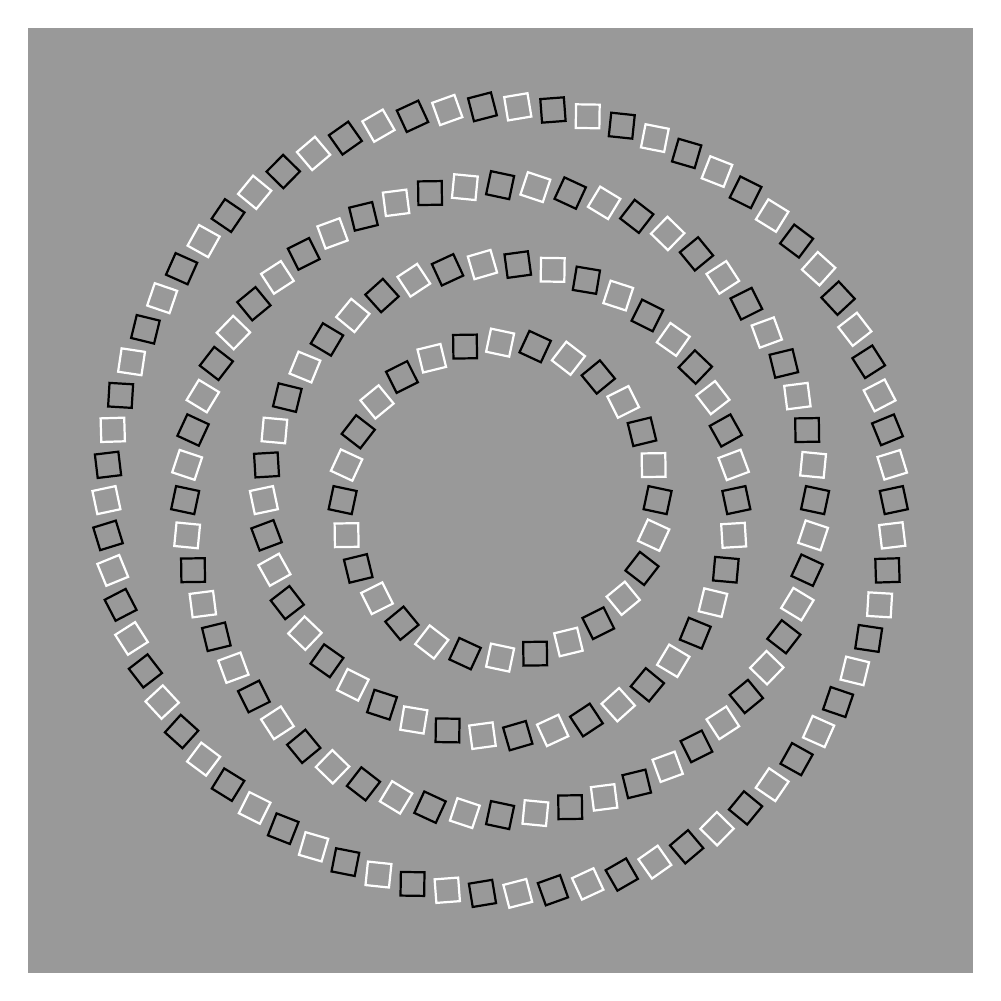
\begin{tikzpicture}
    \fill[color=black!40!white] (-6,-6) rectangle (6,6);
    \foreach \n/\r/\twist in {70/5/12,56/4/-12,42/3/12,28/2/-12}{
            \foreach \m in {1,3,...,\n}
            \draw [thick,color=white,shift={(360/\n*\m:\r)},rotate=\twist+360/\n*\m]
            (-.15,-.15) rectangle (.15,.15);
            \foreach \m in {2,4,...,\n}
            \draw [thick,color=black,shift={(360/\n*\m:\r)},rotate=\twist+360/\n*\m]
            (-.15,-.15) rectangle (.15,.15);
        }
\end{tikzpicture}

\end{document}